% Options for packages loaded elsewhere
\PassOptionsToPackage{unicode}{hyperref}
\PassOptionsToPackage{hyphens}{url}
%
\documentclass[
]{article}
\usepackage{amsmath,amssymb}
\usepackage{lmodern}
\usepackage{iftex}
\ifPDFTeX
  \usepackage[T1]{fontenc}
  \usepackage[utf8]{inputenc}
  \usepackage{textcomp} % provide euro and other symbols
\else % if luatex or xetex
  \usepackage{unicode-math}
  \defaultfontfeatures{Scale=MatchLowercase}
  \defaultfontfeatures[\rmfamily]{Ligatures=TeX,Scale=1}
\fi
% Use upquote if available, for straight quotes in verbatim environments
\IfFileExists{upquote.sty}{\usepackage{upquote}}{}
\IfFileExists{microtype.sty}{% use microtype if available
  \usepackage[]{microtype}
  \UseMicrotypeSet[protrusion]{basicmath} % disable protrusion for tt fonts
}{}
\makeatletter
\@ifundefined{KOMAClassName}{% if non-KOMA class
  \IfFileExists{parskip.sty}{%
    \usepackage{parskip}
  }{% else
    \setlength{\parindent}{0pt}
    \setlength{\parskip}{6pt plus 2pt minus 1pt}}
}{% if KOMA class
  \KOMAoptions{parskip=half}}
\makeatother
\usepackage{xcolor}
\usepackage{longtable,booktabs,array}
\usepackage{calc} % for calculating minipage widths
% Correct order of tables after \paragraph or \subparagraph
\usepackage{etoolbox}
\makeatletter
\patchcmd\longtable{\par}{\if@noskipsec\mbox{}\fi\par}{}{}
\makeatother
% Allow footnotes in longtable head/foot
\IfFileExists{footnotehyper.sty}{\usepackage{footnotehyper}}{\usepackage{footnote}}
\makesavenoteenv{longtable}
\usepackage{graphicx}
\makeatletter
\def\maxwidth{\ifdim\Gin@nat@width>\linewidth\linewidth\else\Gin@nat@width\fi}
\def\maxheight{\ifdim\Gin@nat@height>\textheight\textheight\else\Gin@nat@height\fi}
\makeatother
% Scale images if necessary, so that they will not overflow the page
% margins by default, and it is still possible to overwrite the defaults
% using explicit options in \includegraphics[width, height, ...]{}
\setkeys{Gin}{width=\maxwidth,height=\maxheight,keepaspectratio}
% Set default figure placement to htbp
\makeatletter
\def\fps@figure{htbp}
\makeatother
\setlength{\emergencystretch}{3em} % prevent overfull lines
\providecommand{\tightlist}{%
  \setlength{\itemsep}{0pt}\setlength{\parskip}{0pt}}
\setcounter{secnumdepth}{-\maxdimen} % remove section numbering
\ifLuaTeX
  \usepackage{selnolig}  % disable illegal ligatures
\fi
\IfFileExists{bookmark.sty}{\usepackage{bookmark}}{\usepackage{hyperref}}
\IfFileExists{xurl.sty}{\usepackage{xurl}}{} % add URL line breaks if available
\urlstyle{same} % disable monospaced font for URLs
\hypersetup{
  hidelinks,
  pdfcreator={LaTeX via pandoc}}

\author{}
\date{}

\begin{document}

\begin{quote}
\textbf{5} Solving Havannah with MCTS

Section 4.6 showed that MCTS is capable of solving non-trivial positions
in reasonable time. This chapter will show several improvements to MCTS
in Castro that make it better suited to solving harder positions.

\textbf{5.1 Monte Carlo Tree Search Solving}

Using MCTS to solve positions, as described in Section 4.6, would be
enough to solve any position, given enough time and memory, but in a
player the goal of the solver is mainly to avoid blunders, not
necessarily to prove that the chosen move is optimal. When solving harder positions, more advanced techniques
are needed to prove the outcome in reasonable time and memory. This
section describes several techniques for reducing the search space,
increasing the search speed and reducing memory requirements.

\textbf{5.1.1} \textbf{Symmetry}

There are 37 cells on a size 4 board, but from the starting position
only 6 of them are distinct. The rest are equivalent by symmetry, since
the board has 6-fold rotational symmetry and 2-fold mirror symmetry. By
storing a Zobrist hash {[}26{]} for each of the 12 possible board
orientations and taking the minimum value as the representative hash,
symmetries can be found and ignored. As stones are placed, the number of
possible symmetries decreases dramatically. Symmetric moves are ignored
for the first five ply at node expansion. After five ply, the cost of
calculating the extra hash values and finding the unique moves becomes
too expensive and so symmetry detection is turned o↵for all later moves.

Note that this does not find transpositions, only one-ply symmetries.
Using a hash table of positions based on their Zobrist hash would turn
the game tree into a directed acyclic graph (DAG), thereby dramatically
reducing the search space, but could also lead to inaccuracies due to
hash collisions.

\textbf{5.1.2} \textbf{Multi-threading}

Solving a position usually takes significantly more e↵ort than merely
making a strong move. Therefore it is important to use as much
computation power as possible. On today's multi-core machines, this
means multi-threading.
\end{quote}

Writing fast and thread-safe code is a challenge. In Castro, the control
thread spawns a pool of player threads, but does not participate in the search.
The player threads each follow a simple state machine that includes the
states: WaitStart, WaitEnd, Running, GarbageCollection and Cancelled.
State up-dates are done using atomic compare-and-swap (CAS) machine
instructions to ensure all state transitions are race-free, and to avoid
the contention associ-ated with locks. Barriers are used to pass control
between the control thread and the player threads, as well as to decide
which of the player threads will be used for garbage collection, as it
is a single threaded procedure.

All updates to values in the MCTS tree are also updated with atomic
instructions. Updating experience or RAVE values are done using atomic
increment instructions. Adding children is done with CAS to update the
value of the chil-dren pointer. If multiple threads attempt to create
the same set of children only one will succeed and the others will
instead do a rollout from the parent node. If multiple threads backup
the outcome of a single node in the tree, a race condition related to
early draw detection (described in Section 5.1.5) is possible, so if the
value has changed unexpectedly, the backup is retried to ensure
correctness.

All the player-threads use the same algorithm and the same parameters,
so without any special handling would make the same choices as they
descend the tree. To encourage the threads to explore di↵erent parts of
the tree, virtual losses{[}27{]} are added as each thread descends the
tree. A virtual loss is a loss that is added to the experience of a node
during the descent phase, before the actual experience occurs. If the
rollout results in a loss, this virtual loss is kept as real experience,
but if the rollout results in a win, it is replaced with the true
experience of a win. This makes the nodes that are currently being
explored appear worse than they actually are, possibly worse than their
siblings, thereby encouraging the other threads to explore the siblings
instead. The virtual losses are added atomically as well.
\end{quote}

Contention between threads must be minimized to maximize speed. One
early

72

\begin{quote}
Chapter 5: Solving Havannah with MCTS

source of contention was generating random numbers for the rollouts. The
rand() function in C++ is very fast in a single threaded environment,
but has a lock that limits thread scalability. To avoid this lock, the
MTRand library1 was modified to use only local state variables. One
instance is used per thread. By having the structure local to each
thread, no lock is needed and memory contention is minimized.

Pondering --- thinking during the opponent's time --- is a simple way of
im-proving the strength of a player, and is easy to implement given the
thread pool described above, but it also makes debugging long running
solving at-tempts easier. Simply move to the starting position, then
enable pondering. The player threads will continue solving in the
background, while the control thread continues to respond to commands,
making it possible to query the state of the player to see the status of
the solving attempt. While this is not necessary for a solver, it was
instrumental in determining why some of the openings were taking so long
to solve.

\textbf{5.1.3} \textbf{Garbage Collection}

When solving a non-trivial position, the size of the tree is likely to
be exceed physical memory. For very hard problems it may be several
orders of magni-tude bigger. However, large portions of the tree are
likely to be irrelevant at any given time so can be thrown away when the
available memory is filled. If the deleted nodes are needed later, they
can be recomputed. Various criteria for which part of the tree can be
thrown away are possible, but the one used here is to discard the
children of solved nodes, as well as the children of nodes that have
fewer than N simulations, with a minimum N of 5. N is increased for the
next round of garbage collection if less than half of the memory is
freed, and decreased if more than half the memory is freed. This method
worked

1
\end{quote}

73

\begin{quote}
Chapter 5: Solving Havannah with MCTS

well as long as N remains reasonably small, say below 100, but as N
grows large, the amount of recomputation increases, increasing the
solving time.

\textbf{5.1.4} \textbf{Memory Management}

Garbage collection, as described in Section 5.1.3, should be run any
time the memory use exceeds the user specified memory limit, thereby
freeing up enough memory to continue, but calculating memory use
accurately is not trivial. Memory use is usually naively calculated as
the number of nodes in the tree multiplied by the node size.
Unfortunately this approach ignores the fact that malloc/free (or
new/delete in C++) have some memory management overhead and tend to
fragment memory over time. This fragmentation leaves pockets of
permanently unusable memory, decreasing the usable available memory.
With what amounts to a fixed node limit, extra memory is needed to
compensate for the unusable memory, thereby exceeding the user specified
memory limit.

During a game, fragmentation is unlikely to make a di↵erence as the run
time is short enough that the fragmentation is a small fraction of total
memory. In a long running solver, however, fragmentation could use up to
half of the available memory, likely leading to a severe performance hit
as the system swaps memory to disk. An overhead as high as 30\% was
observed in practice. To avoid this, a compacting tree was implemented.
It periodically rearranges the nodes in the tree to avoid fragmentation,
while allowing the full memory to be used. Conceptually this is similar
to the compacting garbage collectors in higher level languages like
Java. Compacting the tree into a contiguous segment of the heap leaves a
contiguous empty section of the heap, allowing a very fast allocation
strategy to be used. It simply returns the pointer to the beginning of
the empty segment, and moves the empty pointer forward by the amount
that was allocated. This is more memory efficient than a normal malloc
call, which uses fixed and inaccurate bucket sizes. It is also faster,
as
\end{quote}

74

\begin{quote}
Chapter 5: Solving Havannah with MCTS

it is simply an atomic increment. Using this allocation strategy means
every byte is accounted for, allowing strong upper bounds on memory
limits. Several of the harder positions would not be solvable without
this compacting tree, at least not without breaking the positions into
smaller subtrees and solving them independently.

\textbf{5.1.5} \textbf{Early Draw Detection}

Checking the game outcome at node expansion, and backing up wins, losses
and draws as described in Section 4.6 is enough to solve any position,
given sufficient time. Certain positions in Havannah lead to many draws,
and can take prohibitively long to solve without more advanced draw
detection. Figure 3.8b shows a board where no wins are possible after
move 31 even if both players cooperate. Without draw detection this
position will take 6! = 720 simulations to enumerate and prove. In a
game this is not important, since its win ratio approaches the correct
value of a draw quickly, but this is not rigorous enough for a solver.

To show that a position is a draw, the three win conditions need to be
checked to see if any wins of that type are possible. Fork and bridge
wins can be detected with the heuristic described in Section 4.8.6:
start a flood fill from each corner and edge for each player. If none of
the empty cells can reach three edges or two corners for a player, then
that player cannot form a fork or a bridge. One player being unable to
form a fork or a bridge does not preclude the other player from doing
so.

Potential rings can be detected by checking for encirclability. A group
of stones that connects to an edge or corner cannot be encircled by the
opponent. Any cell that is next to a group that connects to an edge or
corner also cannot be encircled by the other player. If no cells can be
encircled, then no rings are possible.
\end{quote}

75

\begin{quote}
Chapter 5: Solving Havannah with MCTS
\end{quote}

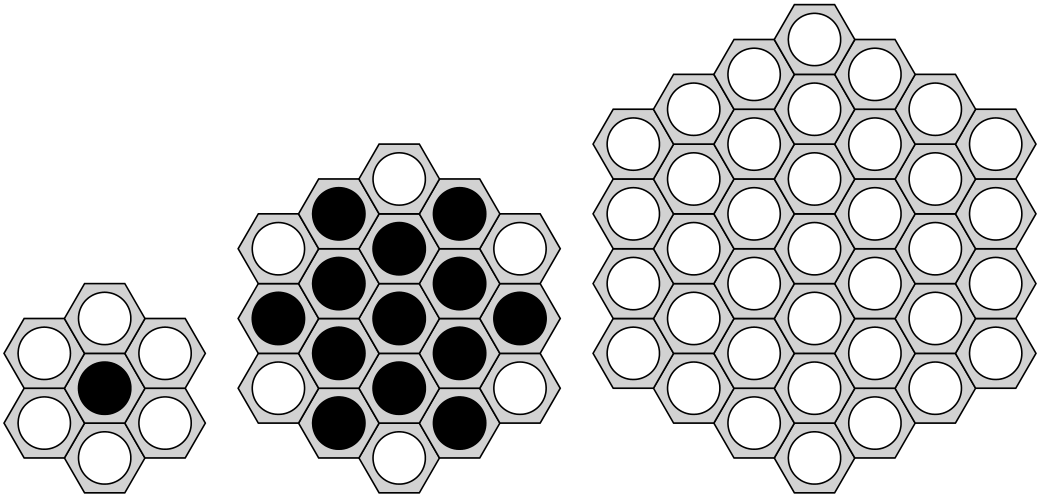
\includegraphics[width=3.61111in,height=1.72222in]{vertopal_cb6790685a974694b23a4a2febc89a47/media/image1.png}

\begin{longtable}[]{@{}
  >{\raggedright\arraybackslash}p{(\columnwidth - 4\tabcolsep) * \real{0.3333}}
  >{\raggedright\arraybackslash}p{(\columnwidth - 4\tabcolsep) * \real{0.3333}}
  >{\raggedright\arraybackslash}p{(\columnwidth - 4\tabcolsep) * \real{0.3333}}@{}}
\toprule()
\begin{minipage}[b]{\linewidth}\raggedright
(a)
\end{minipage} & \begin{minipage}[b]{\linewidth}\raggedright
(b)
\end{minipage} & \begin{minipage}[b]{\linewidth}\raggedright
(c)
\end{minipage} \\
\midrule()
\endhead
\bottomrule()
\end{longtable}

\begin{quote}
Figure 5.1: (a) Solution to size 2 (b) Solution to size 3 (c) Solution
to size 4. The colour of a piece represents the winner if white makes
the first move in that position. No openings lead to a draw.

If no forks, bridges or rings are possible for a player, then that
player cannot win, and so should force a draw if possible. If both
players' best outcome is a draw, then that position is a proven draw.

More advanced techniques of draw detection based on virtual connections
could detect draws much earlier, possibly as early as move 20 in Figure
3.8c, but these techniques have not been explored. The speedup from the
techniques described here may not be as large as 6! for all positions,
but it is still at least an order of magnitude for most early draws.

\textbf{5.2 Solution to Havannah Sizes 2, 3 and 4}

The perfect play solutions to board sizes 2, 3 and 4 are shown in this
sec-tion and in Figure 5.1 in particular. The colour of the piece
represents the player that will win the game if white makes the first
move on that cell. The subsections describe the proofs in more detail.
\end{quote}

76

\end{document}
